\documentclass[conference]{IEEEtran}
\IEEEoverridecommandlockouts
\usepackage{cite}
\usepackage{graphicx}
\usepackage{booktabs}
\usepackage{tabularx}
\usepackage{array}
\usepackage{url}
\usepackage{placeins}
\newcommand{\NA}{\textsc{NA}}
\newcommand{\E}{\textsc{E}}
\newcommand{\N}{\textsc{N}}
\newcommand{\EN}{\textsc{EN}}

\begin{document}
\title{Conditional Post-Alert OT Investigation: Fixed-Budget Evidence Views, Claim Support, and Substantive Coverage}
\author{
\IEEEauthorblockN{PoTing Lu\IEEEauthorrefmark{1},
Eric Mao\IEEEauthorrefmark{1}\thanks{Corresponding author: Eric Mao.}, and
Shih-Hao Chang\IEEEauthorrefmark{2}}
\IEEEauthorblockA{\IEEEauthorrefmark{1}\textit{AvocadoAI Co., Ltd.}, Taipei, Taiwan; eric.mao@mail.avocadolab.ai\\
\IEEEauthorrefmark{2}\textit{Department of Computer Science and Information Engineering,}\\
\textit{National Taipei University of Technology}, Taipei, Taiwan\\
sh.chang@ntut.edu.tw}
}
\maketitle

\begin{abstract}
Process-aware operational technology (OT) detectors can identify anomalous intervals, but an alert alone does not establish command execution, physical completion, causation, or compromise. We study a narrower downstream question: conditional on an externally supplied event scope and time anchor, how do claim support and substantive question coverage differ across fixed-budget evidence views and publication conditions? On 32 preselected Sherlock v3 events, using one hosted model snapshot, three planned repetitions, and one reviewer, we compare 64-record electrical/process-only and network-only configurations with an equal-split 32+32 configuration. The claim-conditioned Complete-Support Rate (CSR) is 0.9261 for the combined configuration versus 0.7500 and 0.7406; however, protocol-exact reference-fact recall is 0.0000 in every view. The citation-required condition has higher CSR than the citation-optional condition (0.9261 versus 0.8723). Exact-replay policy filtering yields checker-aligned Citation Precision and CSR of 1.0000, while Q1--Q6 Substantive Coverage falls from 0.7760 to 0.5278 and required-withholding recall is 0.3344. Because the same frozen policy filters and scores claims, the perfect retained-set scores demonstrate policy consistency, not independent factual validity. These selected-case results provide a conditional, same-policy support--coverage comparison rather than evidence of end-to-end detection, complete incident reconstruction, local-deployment feasibility, or analyst utility.
\end{abstract}
\begin{IEEEkeywords}
operational technology, incident investigation, evidence grounding, large language models, claim support, selective publication
\end{IEEEkeywords}

\section{Introduction}
Process-aware operational technology (OT) detection is well established across subspace, invariant, sequence, rule-based, and state-space methods \cite{aoudi2018pasad,feng2019invariants,kim2020seq2seq,wolsing2022simple,wolsing2025geco}. Sherlock compares their detected-attack, false-alarm, and detection-time trade-offs and identifies \emph{actionability}---helping operators understand and localize an alarm---as an open problem \cite{wagner2025sherlock}. These metrics answer whether and when an alarm is raised; they do not determine what may responsibly be concluded from the evidence available afterward.

The distinction matters in OT. A network request does not establish execution, an acknowledgement does not establish physical completion, and temporal co-occurrence does not establish causation, intent, compromise, or attribution. Post-alert reporting must therefore separate observable records, evidence-supported relationships, qualified interpretations, and unresolved questions. It must also avoid treating a highly supported but narrow claim set as a complete incident reconstruction.

We evaluate a controlled, event-conditioned stage. In deployment, a detector, operational alert, or analyst would supply a scope $W_e$ and anchor $t_0$; in this experiment, the evaluator supplies the same inputs to every applicable condition. The pipeline exposes a fixed evidence view and budget, creates evidence-linked claims, and applies one frozen publication policy (Fig.~\ref{fig:architecture}). These oracle-like inputs permit paired downstream comparison but remove event selection, detector timing error, false-alert burden, and window estimation from the experiment. Evaluator references are scoring-only. The study also specifies evidence scoping and provenance requirements, but it does not evaluate production authorization, local inference, egress enforcement, or analyst benefit.

Our contributions are methodological and empirical measurements rather than a new detector or verifier architecture \cite{zhou2026eviguard}: (1) an explicit operationalization of OT claim-support boundaries that separates observation from execution, causation, and security conclusions; (2) a fixed-total-budget comparison of electrical/process-only (\E; 64 records), network-only (\N; 64 records), and equal-split combined (\EN; 32+32 records) configurations across evidence availability, retrieval, substantive question coverage, Complete-Support Rate (CSR), and protocol-exact matching; and (3) an exact-replay audit that reports same-policy violation removal together with lower substantive coverage and incomplete required withholding. These stages are not interchangeable: support among generated claims cannot substitute for reference-fact recall, and consistency after same-policy filtering cannot establish factual correctness.

Accordingly, \textbf{RQ1} asks how the three fixed-budget evidence configurations differ in retrieval, protocol-exact reference-fact recall, Q1--Q6 Substantive Coverage, and claim-conditioned support. \textbf{RQ2} asks how citation-optional and citation-required generation differ under the same \EN{} configuration. \textbf{RQ3} asks how exact-replay filtering with the same frozen policy changes checker-aligned support and substantive coverage, and characterizes explicit withholding remaining after filtering. Metrics are interpreted jointly; none is treated as end-to-end investigation accuracy.

\section{Background and Related Work}
\subsection{Detection, Alert Handoff, and OT Response}
Process-aware monitoring is well established \cite{rehman2024processaware}. Representative mechanisms include departure-based monitoring and learned invariants \cite{aoudi2018pasad,feng2019invariants}, learned next-state prediction \cite{kim2020seq2seq}, simple process rules \cite{wolsing2022simple}, and comprehensible state-space models \cite{wolsing2025geco}. Under a common but narrow operating point, Sherlock's Table~3 re-evaluates them on 18 attacks in its heavily filtered 01-Basic scenario \cite{wagner2025sherlock}. These are upstream operating-point references, not baselines for downstream CSR or Substantive Coverage: aggregate alarm results cannot replace detector-emitted windows in an end-to-end evaluation.

Cross-domain alert correlation and OT response frameworks already combine detection with broader investigation and coordination \cite{koucham2022crossdomain,smith2021air4ics,staves2022incidentresponse}. Our study isolates only the evidence-to-report portion after a common supplied handoff; it does not evaluate detection quality, organizational response, remediation, or case-management utility.

\subsection{LLMs for Cybersecurity Investigation}
Retrieval-augmented large language models (LLMs) have been evaluated for incident analysis \cite{cadet2026retrieval}, and Cognitive SOC links alert enrichment with evidence-backed narrative generation \cite{sheikhi2025cognitive}. Dehing et al. study local-LLM forensic reporting because privacy can favor authority-controlled hardware, yet still find citation and chronology limitations \cite{dehing2026structured}. OT data-governance guidance likewise motivates bounded evidence interfaces \cite{cisa2025secureaiot}; our public-data, hosted-model experiment does not evaluate locality. Citation correctness also differs from faithful reliance on a source \cite{wallat2025correctness}.

EviGuard is a directly relevant industrial precedent, combining typed claims, provenance, deterministic verifiers, and a response gate \cite{zhou2026eviguard}; we do not claim those mechanisms as architectural novelty. We instead measure fixed-budget \E/\N/\EN{} configurations, passive OT observation semantics, and substantive question coverage before and after exact replay. CSR is claim-conditioned rather than report completeness, while Q1--Q6 Substantive Coverage is report-internal rather than input-level selective-prediction coverage \cite{wen2025know}; two operating points do not define a calibrated frontier.

\section{Conditional Problem Formulation and Study Workflow}
\subsection{Oracle-Conditioned Scope and Evidence Views}
For event $e$, the evaluator supplies a fixed scope $W_e$ and anchor $t_0$, shared by all applicable conditions. Because an evaluated detector does not produce these inputs and they localize an already selected event, we treat them as oracle-like conditioning inputs. They support controlled downstream comparison but are not outputs or scored outcomes. Let $A_e^{\E}=E_e\cup M_e^{\E}$, $A_e^{\N}=N_e\cup M_e^{\N}$, and $A_e^{\EN}=E_e\cup N_e\cup M_e^{\EN}$ denote the complete eligible pre-retrieval views, where each $M_e^v$ contains only the sanitized static mappings permitted for view $v$. Retrieval produces a budgeted, model-visible bundle $B_{e,c}\subseteq A_e^v$: 64 \E{} records, 64 \N{} records, or 32 \E{}+32 \N{} records. Evaluator references $G$ are excluded from every $A_e^v$ and $B_{e,c}$. The task is event-conditioned evidence-to-report generation with a protocol-exact fact-recall diagnostic, not detection, window estimation, or end-to-end incident reconstruction.

The evaluation separates three targets: recovery of evaluator reference facts, support among claims selected by the generator, and policy consistency of the retained set. Protocol-Exact Fact Recall measures the first, CSR the second, and checker-aligned Citation Precision and CSR after exact replay measure the third. Substantive Coverage and withholding describe the content that remains and the restraint made explicit. A favorable later-stage value cannot substitute for failure at an earlier target.

\begin{figure*}[t]
\centering
\IfFileExists{figures/figure1_system_architecture.pdf}{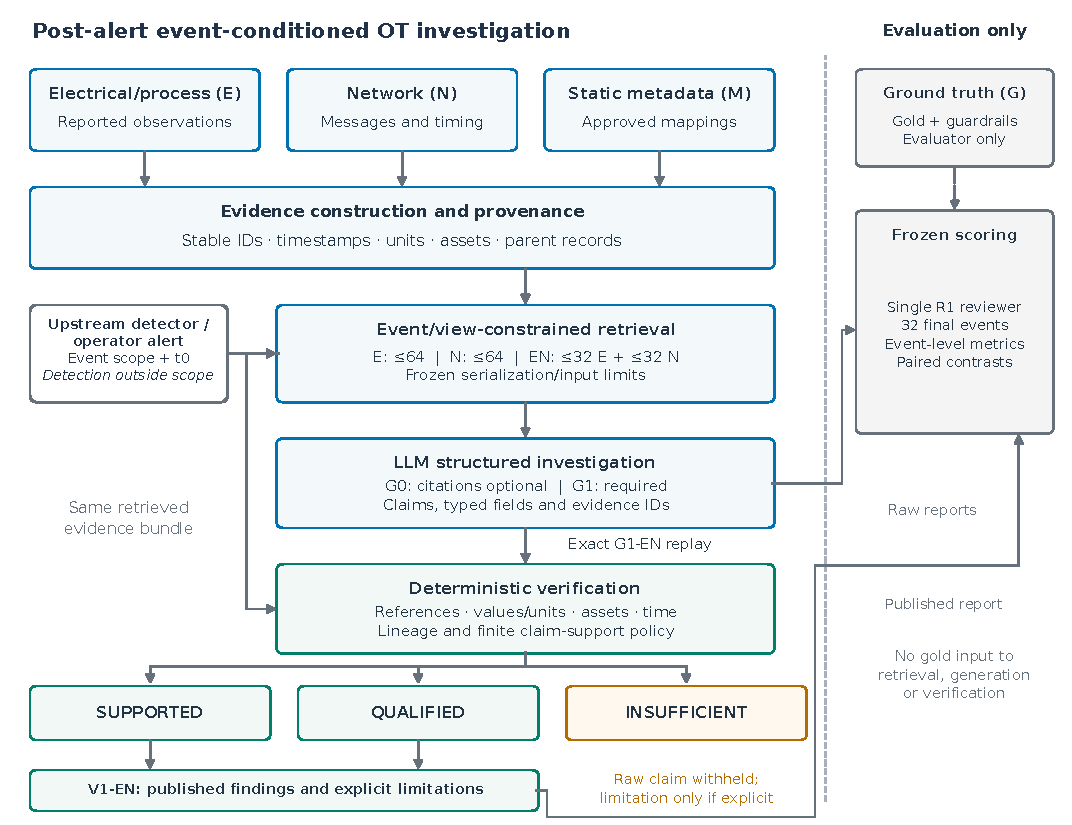
\includegraphics[width=0.88\textwidth]{figures/figure1_system_architecture.pdf}}{\resizebox{0.88\textwidth}{!}{\fbox{\rule{0pt}{396pt}\rule{514.8pt}{0pt}}}}
\caption{Conditional evidence-to-report flow. Scope and anchor are supplied; skill and boundary boxes are deployment interpretations, not evaluated access-control mechanisms. Upstream detectors are external alternatives \cite{aoudi2018pasad,feng2019invariants,kim2020seq2seq,wolsing2022simple,wolsing2025geco}; detector handoff and production enforcement are not evaluated. Evaluator references are scoring-only.}
\label{fig:architecture}
\end{figure*}

\subsection{Deployment Interpretation: Procedures and Case Trace}
An \emph{investigation skill} denotes a versioned procedure contract---inputs, permitted evidence view, output schema, provenance, stop/unknown conditions, and review state---not autonomous authority. A prompt instantiates a procedure but grants no access; case-scoped tools, identity controls, and egress policy would need to enforce least privilege \cite{rose2020zerotrust}. Log and packet content remain untrusted data.

The proposed case trace records alert scope, evidence identifiers and lineage, claims and dispositions, unresolved gaps, policy version, and review state for replay and handoff. The experiment holds scope, view, and budget fixed and implements stable identifiers, reference isolation, a frozen policy, and exact replay. It does not evaluate authorization, sandboxing, egress, tamper resistance, or production case management; these elements are deployment requirements rather than empirical contributions.

\subsection{Claim Semantics and Evidence Representation}
Evidence records retain stable identifiers, timestamps, assets, units, source fields, and transformation lineage. Claim semantics constrain wording to the observation: a network record may support that a command-type request was observed; approved address metadata may support that it targeted a control point mapped to asset $x$. Neither proves asset execution. A response supports that an acknowledgement was observed, not physical completion. Electrical/process records support reported values and changes, not hidden physical truth or network causation. Timestamp ordering supports temporal association, not causality. Claims of intent, successful compromise, and attribution require support beyond these observations.

Table~\ref{tab:claims} gives representative boundaries. The LLM produces structured claims and evidence identifiers from retrieved records; it does not receive evaluator labels. A fixed view and evidence budget constrain retrieval. Citation-required output is compared with citation-optional output under otherwise fixed conditions.

\begin{table*}[t]
\caption{Representative claim-support boundaries}
\label{tab:claims}
\centering\footnotesize
\begin{tabularx}{\textwidth}{@{}lXX@{}}
\toprule
Claim type & Evidence sufficient for bounded wording & Unsupported promotion\\
\midrule
Network command & Command-type request observed; mapping permits ``addressed to a control point mapped to $x$'' & Command executed; asset physically acted\\
Acknowledgement & Protocol response observed & Physical operation completed\\
Reported value/change & Electrical/process observation(s), compatible units, supported arithmetic & Hidden physical truth; network activity caused change\\
Asset/time relation & Approved mapping and timestamps establish relation/order & Compromise; temporal association implies causation\\
Security conclusion & Only a claim-specific policy with sufficient visible support & Intent, successful compromise, or attribution from observation alone\\
\bottomrule
\end{tabularx}
\end{table*}

\subsection{Evidence-Bounded Claim Generation}
For each event and view, retrieval selects records within the externally supplied scope and frozen input limits. The LLM structures observable facts, relationships, qualified interpretations, and unresolved questions. Substantive claims may cite only evidence IDs visible at generation time. Evaluator reference facts, attack labels, scenario descriptions, and hidden simulator state are inaccessible.

\subsection{Same-Policy Publication Filtering}
The deterministic checker applies the frozen evidence-support policy to visible references, numerical values and units, asset mappings, time ordering, transformation lineage, and claim-specific support requirements. It assigns supported, qualified, or insufficient dispositions; publication filtering retains policy-admissible wording and suppresses insufficient claims. Required Withholding Recall and Withholding Precision, defined below, score only explicit qualification or withholding statements, not silent suppression. Because the same policy also defines checker-aligned scoring, retained-set scores measure construction consistency, not independent verifier accuracy, policy validity, truth, or causal inference. An undefined metric is reported as \,\NA, not numerical zero; absence of support is not evidence of a benign event.

\section{Experimental Methodology}
\subsection{Dataset and Event Set}
The study uses Sherlock v3, a Wattson power-grid co-simulation dataset with IEC 60870-5-104 traffic and electrical/process observations \cite{wagner2025sherlock,sherlockv3}. The 16 development events are drawn from 01-Basic. The 32 final events comprise 18 Semiurban and 14 Rural events, balanced across 16 cyber and 16 benign cases. Within frozen scenario-by-family quotas, a predeclared greedy maximin rule over squared distances between within-scenario midranks of observable features, with a SHA-256 tie-break, selected events without classifier predictions or LLM results. The data had previously been inspected, so this is a constructed benchmark rather than an untouched confirmation sample or an estimate of operational prevalence. Event identifiers were frozen before final generation. The final set is scored against reviewed event facts and unresolved-conclusion opportunities; evaluator-only material is separated from model input. The target of inference is this finite selected set under its frozen inputs, not the Sherlock population or operational alert prevalence. Artifacts, event identifiers, prompts, policies, manifests, and scoring code are available in the project repository.\footnote{\url{https://github.com/CHPIYR2/ICIT2027}}

\subsection{Experimental Conditions}
Table~\ref{tab:conditions} summarizes the cells. All generative cells use one fixed hosted model snapshot (gpt-4.1-2025-04-14), condition-specific prompt variants frozen before evaluation, a common schema, temperature 0, a 24,576-token maximum output, no supplied seed, no tools, automatic input truncation disabled, and three planned repetitions per event; hosted-versus-local inference is not a study factor. G0 and G1-EN differ only in the citation requirement; G1-E, G1-N, and G1-EN share the citation-required prompt variant and differ only in evidence view and allocation. RQ1 holds the total retrieval budget at 64 records: 64 E, 64 N, or a 32 E + 32 N allocation for EN, with serialized-input limits also fixed. The contrasts therefore compare equal-total-budget configurations, not the causal effect of adding a modality. D0 checks deterministic export and scoring behavior; it is not commensurate with the generative cells, enters no RQ contrast, and cannot establish LLM benefit. The study compares controlled configurations of one pipeline and includes no independent method-level investigation baseline. G1-E has three provider-incomplete repetitions (93 complete deliveries of 96); those deliveries are missing, but all 32 event means remain defined. V1-EN is exact replay of raw G1-EN: no additional LLM generation.

\begin{table}[!ht]
\caption{Experimental condition summary}
\label{tab:conditions}
\centering\footnotesize
\begin{tabularx}{\columnwidth}{@{}l l X@{}}
\toprule
Cell & View & Role / policy\\
\midrule
D0 & EN & Protocol-integrity reference; not a performance baseline\\
G0 & EN & LLM; citations optional (RQ2)\\
G1-E & E & LLM; citations required (RQ1)\\
G1-N & N & LLM; citations required (RQ1)\\
G1-EN & EN & LLM; citations required (RQ1--RQ3)\\
V1-EN & EN & Exact G1-EN replay; same-policy publication filter (RQ3)\\
\bottomrule
\end{tabularx}
\end{table}

\subsection{Reference Review and Metric Interpretation}
One reviewer (R1) constructed the sealed evaluator reference set and performed all subjective output judgments under the frozen review contract, completing 477 ledgers: 381 valid generative deliveries (96 G0, 93 G1-E, 96 G1-N, and 96 G1-EN) and 96 exact-replay V1 ledgers. Reference facts, opportunities, and the matching policy were committed before output review. A later append-only correction excluded D0 from subjective review scope without changing research-cell scoring semantics. No dual annotation or adjudication was performed, so inter-annotator agreement is unavailable; we make no claim of condition blinding. Outcomes are therefore R1-rubric-conditioned rather than independently validated semantic ground truth.

Let $G_e$ be the R1 reference-fact set and $G_{e,v}\subseteq G_e$ the facts supportable from the complete eligible pre-retrieval view $A_e^v$. Protocol-Exact Fact Recall is the fraction of $G_e$ recovered by R1 whole-assertion matches under the frozen proposition, field, numerical, and evidence-visibility criteria. View-Conditional Exact Recall applies the same numerator rule with denominator $|G_{e,v}|$. Retrieval Recall is the number of facts in $G_{e,v}$ whose complete required support set was retrieved, divided by $|G_{e,v}|$. No separate relaxed semantic-equivalence or partial-credit metric was prespecified.

Q1--Q6 Substantive Coverage is the fraction of six questions---network activity, process observations, assets, timeline, cross-source relations, and bounded security interpretation---for which R1 identifies at least one substantive, supported assertion; Q7 separately records unknowns. Coverage is neither fact recall nor demonstrated analyst utility. Citation Precision divides generated evidence-role citation pairs whose identifier exists, is visible, and supports the assigned role by all generated citation pairs. Before claim-level scoring, R1 splits compound text into atomic substantive assertions and de-duplicates repeated assertions. CSR divides de-duplicated atomic substantive assertions completely supported by a valid support set contained in the assertion's own citations by all de-duplicated atomic substantive assertions; evaluator-added evidence cannot repair an incomplete cited set. The Unsupported Security-Claim Rate (USCR) divides unsupported security-sensitive substantive assertions by all security-sensitive substantive assertions; both security sensitivity and support status are R1 judgments. Required Withholding Recall is the fraction of R1-annotated opportunities for which the output correctly qualifies or withholds the action, scope, and reason. Withholding Precision is the fraction of explicit qualification or withholding actions that are correct. Each ratio is \NA{} when its denominator is zero. Because several denominators depend on generated output, claim-conditioned rates may change through support quality, claim selection, or both. Metrics are computed per repetition, averaged within event, and then macro-averaged; D0 is excluded from primary RQ comparisons.

\subsection{Conditional Estimand and Statistical Analysis}
For metric $m$, let $\bar m_{e,c}$ be the mean across valid repetitions for event $e$ under condition $c$. Fixed-denominator contrasts report the finite-set event-macro difference $\Delta^{(32)}_{a,b}(m)=32^{-1}\sum_e(\bar m_{e,a}-\bar m_{e,b})$; claim-conditioned metrics use only event pairs with both denominators defined, and the paired count is reported. The estimand is conditional on the selected events, supplied $W_e$ and $t_0$, retrieval allocation, model, prompt/schema, policy, and reviewer rubric.

We report 95\% scenario-stratified percentile bootstrap stability intervals from 2,000 resamples, seed 20270922. Claims and repetitions are not independent samples. These intervals summarize sensitivity to the composition of the selected cases; they do not incorporate event-selection, single-reviewer, or generation uncertainty and are not population-level or cross-site generalization intervals.

\FloatBarrier
\section{Results}
Under the frozen matcher, Protocol-Exact Fact Recall and View-Conditional Exact Recall are 0.0000 for \E, \N, and \EN. This primary negative result has a floor and does not distinguish the configurations. Because no separate relaxed semantic-equivalence or partial-credit measure was prespecified, the data cannot determine whether a nonmatch omitted a reference fact or expressed related content that failed the whole-assertion field and numerical criteria. The remaining metrics characterize visible support opportunities, retrieval, question-level substantive coverage, and support among produced claims; none substitutes for reference-fact recall. Per event, the mean numbers of view-supportable reference facts and facts with complete support retrieved are 9.0 and 1.0 for \E, 3.5 and 1.0 for \N, and 14.0 and 3.125 for \EN; no valid RQ1 generative output matches a fact under the frozen criterion. Table~\ref{tab:results} summarizes outcomes and paired contrasts.

\begin{table*}[!t]
\caption{Event-level macro means and paired 95\% scenario-stratified percentile bootstrap stability intervals for the 32 selected events. Claim-conditioned means use defined events only.}
\label{tab:results}
\centering\scriptsize
\begin{tabularx}{\textwidth}{@{}l l X X@{}}
\toprule
RQ & Metric & Condition means & Paired contrast / denominator note\\
\midrule
1 & Protocol-Exact Fact Recall & E 0.0000; N 0.0000; EN 0.0000 & EN$-$E 0.0000 [0.0000, 0.0000]; EN$-$N 0.0000 [0.0000, 0.0000]\\
1 & View-Conditional Exact Recall & All 0.0000 & No valid RQ1 generative output matches a reference fact under the frozen criterion\\
1 & Retrieval Recall & E 0.1111; N 0.3500; EN 0.2188 & EN$-$E +0.1076 [0.0920, 0.1207]; EN$-$N $-$0.1313 [$-$0.1938, $-$0.0714]\\
1 & Q1--Q6 Substantive Cov. & E 0.7691; N 0.5972; EN 0.7760 & EN$-$E +0.0069 [$-$0.0686, 0.0747]; EN$-$N +0.1788 [0.0885, 0.2674]\\
1 & Citation Precision & E 0.9901; N 0.9589; EN 0.9949 & EN$-$E +0.0048 [$-$0.0048, 0.0192]; EN$-$N +0.0360 [0.0186, 0.0565]\\
1 & Complete-Support Rate & E 0.7500; N 0.7406; EN 0.9261 & EN$-$E +0.1761 [0.1449, 0.2030]; EN$-$N +0.1856 [0.1480, 0.2208]\\
2 & Citation Precision; CSR; Substantive Cov. & G0 0.9907; 0.8723; 0.7465. G1-EN 0.9949; 0.9261; 0.7760 & G1-EN$-$G0: CSR +0.0539 [0.0287, 0.0794]; Citation Precision +0.0042 [$-$0.0027, 0.0121]; coverage +0.0295 [$-$0.0313, 0.0903]\\
2 & USCR & G0 0.0000; G1-EN 0.0000 when defined & Sparse: G0 13 defined/19 NA events; G1-EN 15 defined/17 NA events; paired denominator 7. No decrease established\\
3 & Citation Precision; CSR & G1-EN 0.9949; 0.9261. V1-EN 1.0000; 1.0000 & V1$-$G1: +0.0051 [0.0015, 0.0092]; +0.0739 [0.0504, 0.0970]\\
3 & Q1--Q6 Substantive Cov. & G1-EN 0.7760; V1-EN 0.5278 & $-$0.2483 [$-$0.2934, $-$0.1979]\\
3 & Withholding; USCR & V1 recall 0.3344; precision 1.0000 on defined events & Precision defined on 27 events (5 NA); G1-EN USCR defined on 15 events, V1 USCR = \NA on all 32\\
\bottomrule
\end{tabularx}
\end{table*}

\begin{figure*}[!t]
\centering
\IfFileExists{figures/figure2_coverage_uscr.pdf}{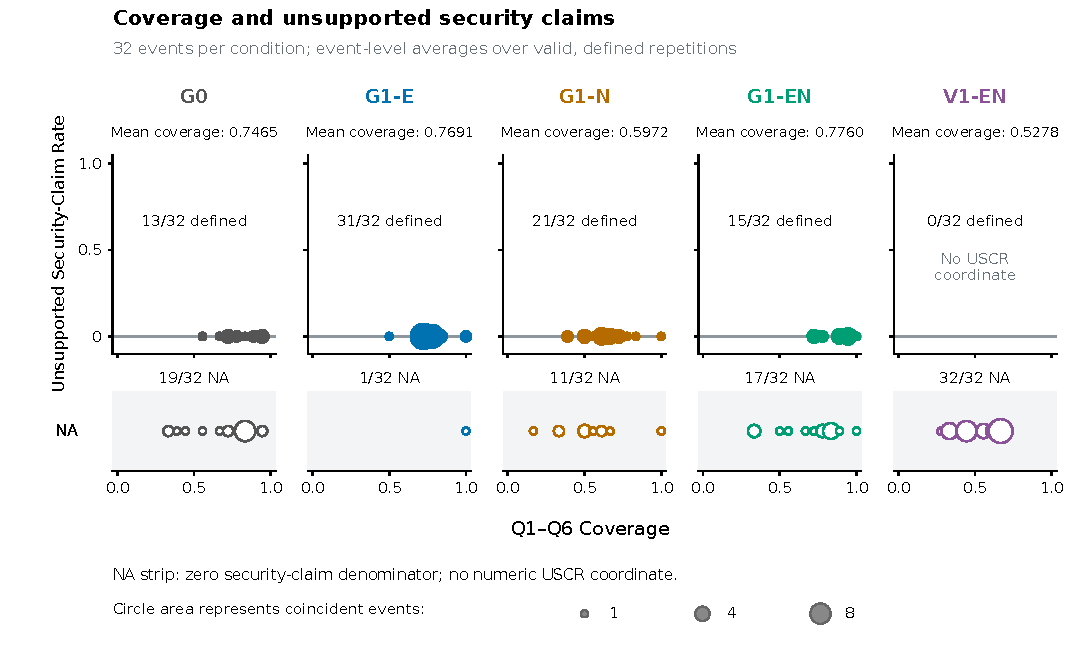
\includegraphics[width=0.96\textwidth]{figures/figure2_coverage_uscr.pdf}}{\resizebox{0.96\textwidth}{!}{\fbox{\rule{0pt}{309.6pt}\rule{514.8pt}{0pt}}}}
\caption{Q1--Q6 Substantive Coverage and USCR by condition. For V1-EN, all 32 security-sensitive assertion denominators are zero; its USCR coordinate is \NA, not zero.}
\label{fig:coverage}
\end{figure*}

\subsection{RQ1---Fixed-Budget Evidence Configurations}
Under the 64-record budget, equal-split \EN{} has higher claim-conditioned CSR than \E{} and \N{} (+0.1761 and +0.1856). Its Substantive Coverage exceeds \N{} (+0.1788); the observed \EN{}--\E{} difference is +0.0069, and its interval crosses zero. Retrieval Recall is higher for \N{} than \EN, although \N{} contains fewer supportable facts; complete support is retrieved for 1.0 reference fact under \N{} and 3.125 under \EN{} on average. These are paired contrasts among allocations that also differ in record composition and information density, not a causal modality-addition effect; every configuration has zero Protocol-Exact Fact Recall.

\subsection{RQ2---Citation Requirement and Claim Portfolio}
The citation-required condition produces a claim portfolio with CSR 0.9261 versus 0.8723 for citation-optional generation (paired $\Delta=+0.0539$, 95\% stability interval [0.0287, 0.0794]). Paired differences in Citation Precision and Substantive Coverage have intervals that cross zero. Because CSR is conditioned on generated substantive claims, the difference may reflect support quality, claim selection, or both; it is neither unconditional report completeness nor a causal estimate of citation effectiveness. USCR is 0.0000 where defined in both conditions, but sparse denominators (13 G0 and 15 G1-EN defined events; seven jointly defined) do not establish a reduction in unsupported security conclusions. G0 is citation-optional, not citation-free.

\subsection{RQ3---Same-Policy Publication Filtering}
V1 applies the frozen policy to exact G1-\EN{} replays and is scored with metrics derived from that policy. After filtering, checker-aligned Citation Precision and CSR are 1.0000 because no policy-detectable violation remains in the retained set. These construction-consistency values do not estimate independent verifier accuracy, factual correctness, or policy validity. Substantive Coverage falls from 0.7760 to 0.5278; Required Withholding Recall is 0.3344 across 32 events, while Withholding Precision is 1.0000 on 27 defined events and \NA{} on five events with no explicit withholding action. R1 identifies no retained security-sensitive substantive assertion, so USCR is \NA{} on all 32 events rather than zero. The result is a paired change in same-policy admissibility and coverage together with the observed post-filter withholding behavior, not proof that filtering makes an investigation safer or more correct.

\section{Discussion and Limitations}
The central finding is separation rather than successful reconstruction. Protocol-exact fact recall is zero in every view, whereas \EN{} has higher CSR among the claims it elects to produce. These outcomes answer different questions: CSR cannot replace reference-fact recall, and no separate relaxed semantic or partial-credit reconstruction measure was collected. Likewise, V1's perfect checker-aligned scores follow same-policy filtering; the informative observation is that they co-occur with a Substantive Coverage decrease from 0.7760 to 0.5278 and required-withholding recall of 0.3344. This is one same-policy admissibility--coverage comparison, not a calibrated frontier or proof of useful, safe investigation.

The same single-reviewer framework underlies reference-fact construction and subjective claim-support judgments. Reviewer interpretation can therefore affect both denominators and outcomes, and the study provides no independent estimate of annotation reliability, semantic correctness, or analyst utility. A second reviewer, blinded semantic matching, and independent scoring of raw and retained claims are required before treating exact nonmatches as semantic failures or policy-admissible claims as factually validated.

Shared oracle-like $W_e,t_0$ inputs preserve downstream comparability but remove detector timing error, false-alert burden, and window uncertainty. Sherlock's Table~3 detectors remain upstream references because their emitted windows are not propagated here. The 32 events come from one co-simulation dataset; the study uses one hosted model, three G1-E repetitions are provider-incomplete, claim-conditioned denominators are sparse, and \E/\N{} may share packet ancestry. The fixed record allocations also confound modality with quota and information density.

Finally, public sanitized data do not test on-premises operation, resource or latency constraints, data residency, authentication, per-procedure authorization, sandbox or egress enforcement, prompt/evidence injection, or tamper-resistant tracing. Those are deployment requirements, not demonstrated properties. Priority validation should add independent review and semantic fact matching, checker challenge cases and alternative policies, matched-budget allocations, and detector-generated true- and false-positive windows before broader model, site, or analyst studies.

\section{Conclusion}
We measured event-conditioned OT report generation on 32 preselected Sherlock v3 events under evaluator-supplied, oracle-like scopes and time anchors. Under a fixed 64-record budget, equal-split \EN{} has higher claim-conditioned, R1-rubric-scored CSR than the evaluated single-view configurations, but none of the scored generative evidence-view configurations matches a reference fact under the frozen protocol-exact criterion. No separate relaxed semantic or partial-credit reconstruction measure was evaluated.

Exact-replay publication filtering makes the retained set consistent with the same policy used to score it while reducing Q1--Q6 Substantive Coverage and leaving many required withholding opportunities unexpressed. The results are selected-case, single-reviewer measurements of one pipeline's configurations and publication policy. They do not establish end-to-end detection value, independent verifier accuracy, factual truth, complete incident reconstruction, local deployment, or analyst benefit.

\bibliographystyle{IEEEtran}
\IfFileExists{references.bib}{\bibliography{references}}{}
\end{document}
